\begin{multicols}{2}
\subsection{Eure Profs}
	Um euch einen kleinen Vorgeschmack auf die Leute zu geben, die euch demnächst mit ihrem Wissen beglücken wollen, seien sie hier kurz aufgeführt:

\subsubsection{Algorithmen und Datenstrukturen}
	%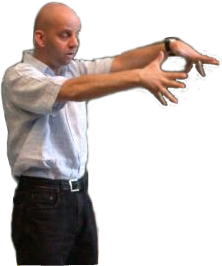
\includegraphics[width=0.7\linewidth]{bilder/dozenten/fekete_frei.png}\\
	\textit{Prof. S\'andor Fekete}

	Diese Vorlesung vermittelt Programmiersprachenunabhängige Konzepte wie Bäume, Listen oder Stacks. Wer nicht weiß, was sich hinter diesen Begriffen verbirgt, sollte auf keinen Fall die Übungen verpassen.

\subsubsection{Programmieren 1}
	%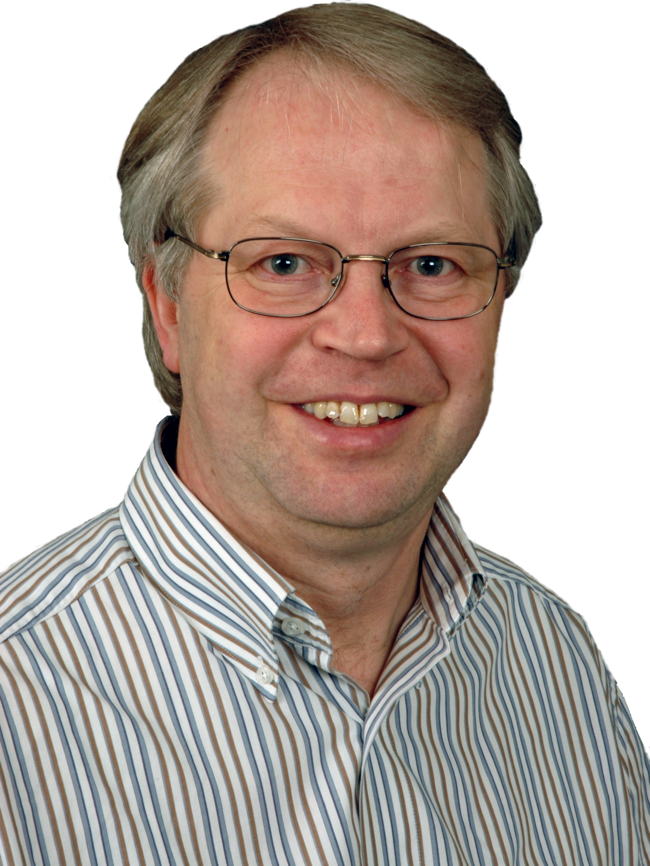
\includegraphics[width=0.6\linewidth]{bilder/dozenten/struck.png}\\
	\textit{Dr. Werner Struckmann}
	
	Programmiert wird hier fast ausschließlich in Java. Wer keine oder nur wenig Erfahrungen mit Java gemacht hat, sollte unbedingt die kleinen Übungen bearbeiten.

\subsubsection{Lineare Algebra}
	%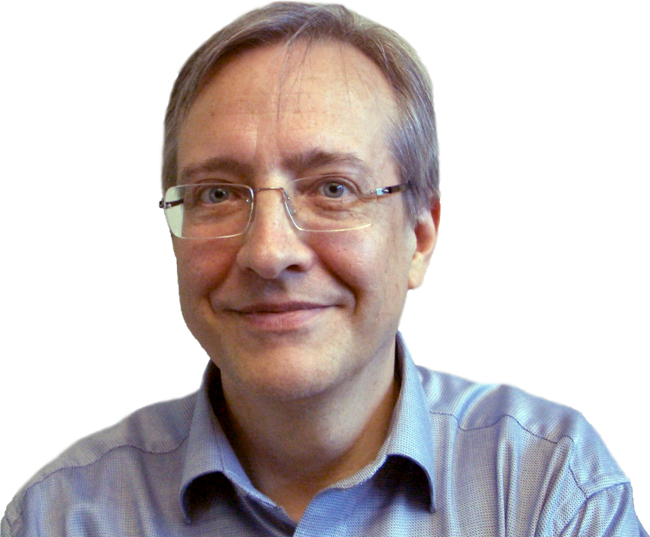
\includegraphics[width=0.8\linewidth]{bilder/dozenten/marten_frei.png}\\
	\textit{Dr. Wolfgang Marten}

	Hier geht es um Vektoren und Matrizen, sowie ein wenig Gruppentheorie. Die übungen sind zwar nicht immer einfach, geben aber einen sehr guten Ausblick auf die Klausur.

\subsubsection{Theoretische Informatik 1}
%	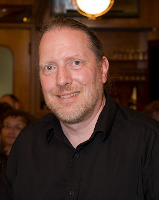
\includegraphics[width=0.6\linewidth]{bilder/dozenten/koslowski.png}\\
	\textit{Dr. Jürgen Koslowski}

	Hier geht es um die formale Sprachen und Automatentheorie. Klingt theoretisch und mathelastig? Ist es auch. Nicht gleich aufgeben, wenn man in der Vorlesung nicht mitkommt, die kleinen Übungen helfen beim Verständnis und bei der Klausurvorbereitung.

\subsubsection{Diskrete Mathematik}

	Diskrete Mathematik handelt von allem, was mit ganzen Zahlen zu tun hat: Fibbonacci-Zahlen, Primzahlen, Modulorechnung, usw. Die Veranstaltung wird von Prof. Arnfried Kemnitz gehalten.

\subsubsection{Wissenschaftliches Arbeiten}
%	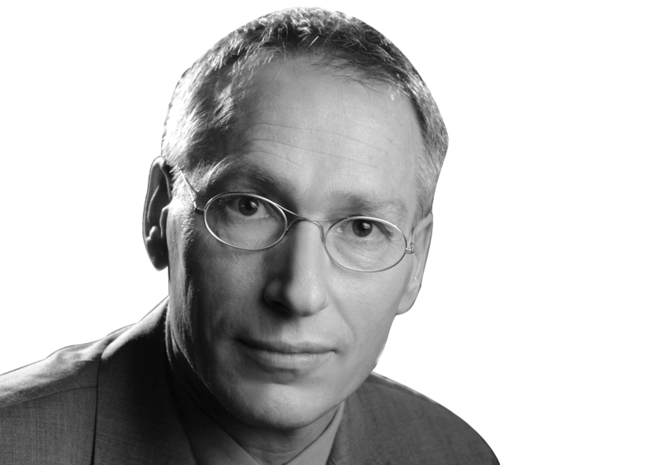
\includegraphics[width=0.9\linewidth]{bilder/dozenten/jung_frei.png}\\
	\textit{Prof. Helmut Jung}
	
	In dem Kurs \emph{wissenschaftliches Arbeiten} lernen die Teilnehmer/-innen, Schritt für Schritt eine wissenschaftliche Arbeit durchzuführen -- beispielsweise eine Bachelorarbeit. Hierzu erfahrt ihr, wie man systematisch vorgeht und welche Methoden man in welchem Schritt verwenden kann. Er ist eine freiwillige Schlüsselqualifikation, die Teilnahme wird aber empfohlen.
\end{multicols}
